\documentclass[12pt]{beamer}


%%%%%%%%%
% Theme %
%%%%%%%%%

\usetheme{metropolis}


%%%%%%%%%%%%
% Packages %
%%%%%%%%%%%%

\usepackage[english]{babel}
\usepackage{sleek/sleek-beamer}

\usepackage{subcaption}


%%%%%%%%%%%%
% Commands %
%%%%%%%%%%%%

\newcommand{\captionsource}[2]{
    \captionsetup{justification=centering}
    \caption*{#1\\\scriptsize\textbf{Source:} \url{#2}}
}


%%%%%%%%%%%%%%
% References %
%%%%%%%%%%%%%%

\addbibresource{references.bib}


%%%%%%%%%%%%%%%%%%
% Title settings %
%%%%%%%%%%%%%%%%%%

\title{Neural style transfer}
\subtitle{Deep learning project}
\author{Maxime Meurisse, Adrien Schoffeniels, Valentin Vermeylen}
\institute{University of Liège}
\date{June 5, 2020}
\titlelogo{resources/others/logo-uliege.pdf}
\framelogo{resources/others/logo-uliege.pdf}


%%%%%%%%%%%%
% Document %
%%%%%%%%%%%%

\begin{document}
    % ----- Title ----- %
    
    \maketitle
    
    % ----- Introduction ----- %
    
    \begin{frame}{Neural style transfer}
        \textbf{Ultimate goal} : merge the style of an image and the content of another image.
        
        \begin{figure}[H]
            \centering
            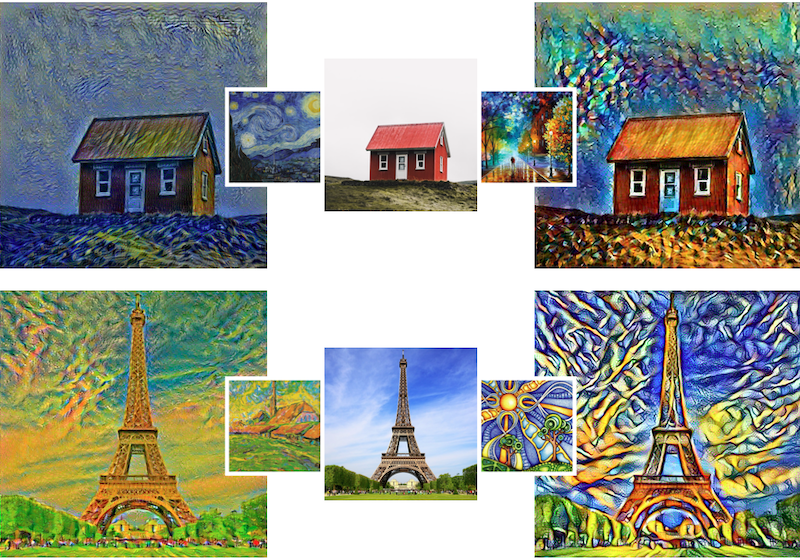
\includegraphics[width=0.65\textwidth]{resources/gatys/gatys-final.png}
            \caption*{Neural style transfer results (Gatys et al. technique)}
        \end{figure}
    \end{frame}
    
    % ----- Plan of the presentation ----- %
    
    \begin{frame}{Plan of the presentation}
        Development of the 2 techniques used :
        
        \begin{itemize}
            \item \emph{A Neural Algorithm of Artistic Style} (Gatys et al., 2015)
            \item \emph{Unpaired Image-to-Image Translation using Cycle-Consistent Adversarial Networks} (Zhu et al., 2017)
        \end{itemize}
        
        and a conclusion.
    \end{frame}
    
    % ----- Gatys et al. ----- %
    
    \section{A Neural Algorithm of Artistic Style (Gatys et al., 2015)}
    
    \begin{frame}{Method}
        \begin{itemize}
            \item Use a (pre-trained) convolutional neural network (CNN)
            \item {\bf Key} : style and content of an image are separable in CNN
            \item Add new layers in the CNN to re-construct images
        \end{itemize}
        
        \begin{figure}[H]
            \centering
            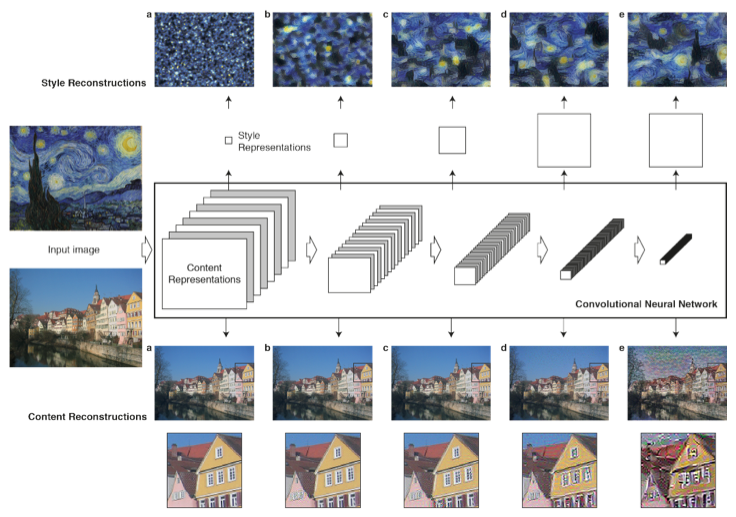
\includegraphics[width=0.55\textwidth]{resources/gatys/method/image-reconstruction-cnn.png}
            \captionsource{Image reconstruction - CNN}{https://arxiv.org/gatys/1508.06576.pdf}
        \end{figure}
    \end{frame}
    
    \begin{frame}{Method - Loss functions}
        $$\mathcal{L}_{total} = \alpha \mathcal{L}_{content} + \beta \mathcal{L}_{style}$$
        where, for a layer $l$,
        $$\mathcal{L}_{\text {content}} = \frac{1}{2} \sum_{i, j}\left(F_{i j}^{l}-P_{i j}^{l}\right)^{2}$$
        and
        $$\mathcal{L}_{\text {style}} = \sum_{l=0}^{L} w_{l} \frac{1}{4 N_{l}^{2} M_{l}^{2}} \sum_{i, j}\left(G_{i j}^{l}-A_{i j}^{l}\right)^{2}$$
        
        \scriptsize{
            \begin{itemize}
                \item $F_{ij}$ and $P_{ij}$, $\in \mathcal{R}^{N_l\times M_l}$ : activation of the $i^{th}$ filter at position $j$ in layer $l$
                \item $G_{ij}$ and $A_{ij}$ : Gram matrices
            \end{itemize}
        }    
    \end{frame}
    
    \begin{frame}{Results}
        Base images used :
        
        \begin{figure}[H]
            \centering
            \begin{subfigure}[b]{0.25\textwidth}
                \centering
                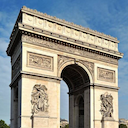
\includegraphics[width=\textwidth]{resources/gatys/inputs/paris.png}
                \caption{Content}
            \end{subfigure}
            \hfill
            \begin{subfigure}[b]{0.25\textwidth}
                \centering
                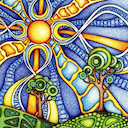
\includegraphics[width=\textwidth]{resources/gatys/inputs/sun-trees.png}
                \caption{Style 1}
            \end{subfigure}
            \hfill
            \begin{subfigure}[b]{0.25\textwidth}
                \centering
                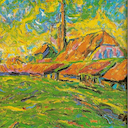
\includegraphics[width=\textwidth]{resources/gatys/inputs/church.png}
                \caption{Style 2}
            \end{subfigure}
        \end{figure}
        
        Evaluation methods :
        
        \begin{itemize}
            \item {\bf qualitative} (human eyes)
            \item quantitative (loss functions : content and style)
        \end{itemize}
    \end{frame}
    
    \begin{frame}
        Different (significant) parameters :
        
        \begin{itemize}
            \item input image
            \item model used
            \item architecture of the model used
            \item weights
            \item added layers
        \end{itemize}
    \end{frame}
    
    \begin{frame}{Input image}
        2 ways to initialize the input image :
        
        \begin{itemize}
            \item copy of content image
            \item noisy content image
        \end{itemize}
    \end{frame}
    
    \begin{frame}
        \begin{figure}[H]
            \centering
            \begin{subfigure}[b]{0.45\textwidth}
                \centering
                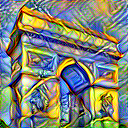
\includegraphics[width=\textwidth]{resources/gatys/inputs/sun-trees-paris-copy.png}
                \caption{Copy of content image}
            \end{subfigure}
            \hfill
            \begin{subfigure}[b]{0.45\textwidth}
                \centering
                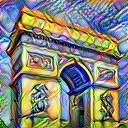
\includegraphics[width=\textwidth]{resources/gatys/inputs/sun-trees-paris-noisy.png}
                \caption{Noisy content image}
            \end{subfigure}
        \end{figure}
        
        Very similar results obtained.
        
        \footnotesize{Copy of content image chosen because smoother results on average.}
    \end{frame}
    
    \begin{frame}{Model used}
        Base model used : {\bf VGG19}
        
        \begin{itemize}
            \item not pre-trained
            \item pre-trained
        \end{itemize}
        
        We also tried :
        
        \begin{itemize}
            \item GoogLeNet
            \item AlexNet
        \end{itemize}
    \end{frame}
    
    \begin{frame}
        \begin{figure}[H]
            \centering
            \begin{subfigure}[b]{0.45\textwidth}
                \centering
                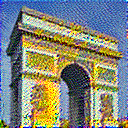
\includegraphics[width=\textwidth]{resources/gatys/models/sun-trees-paris-notpretrained.png}
                \caption{VGG19 : not pre-trained}
            \end{subfigure}
            \hfill
            \begin{subfigure}[b]{0.45\textwidth}
                \centering
                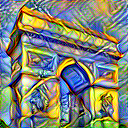
\includegraphics[width=\textwidth]{resources/gatys/models/sun-trees-paris-pretrained.png}
                \caption{VGG19 : pre-trained}
            \end{subfigure}
        \end{figure}
        
        Pre-trained model gives much better results than the non pre-trained model.
        
        \footnotesize{VGG19 pre-trained model chosen.}
    \end{frame}
    
    \begin{frame}
        \begin{figure}[H]
            \centering
            \begin{subfigure}[b]{0.45\textwidth}
                \centering
                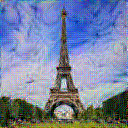
\includegraphics[width=\textwidth]{resources/gatys/models/googlenet.png}
                \caption{GoogLeNet : pre-trained}
            \end{subfigure}
            \hfill
            \begin{subfigure}[b]{0.45\textwidth}
                \centering
                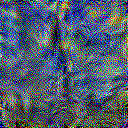
\includegraphics[width=\textwidth]{resources/gatys/models/alexnet.png}
                \caption{AlexNet : pre-trained}
            \end{subfigure}
        \end{figure}
        
        Very bad results obtained.
        
        \footnotesize{Certainly due to a too simple (AlexNet) or too complex/unability to modify submodules (GoogLeNet) architecture.}
    \end{frame}
    
    \begin{frame}{Architecture of the model used}
        VGG19 uses \textbf{max} pooling layers by default.
        
        \begin{figure}[H]
            \centering
            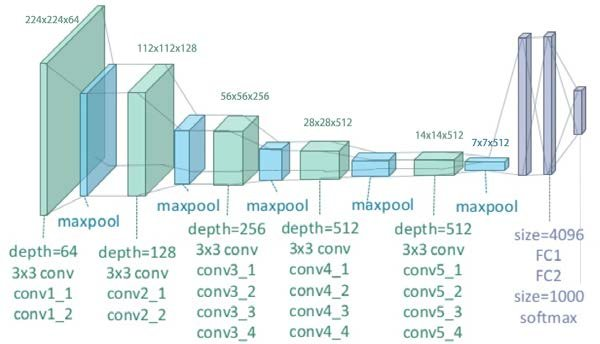
\includegraphics[width=0.5\textwidth]{resources/gatys/architecture/vgg19-architecture.png}
            \captionsource{VGG19 architecture}{https://mc.ai/style-transfer-of-images-with-cnn-in-pytorch/}
        \end{figure}

        Authors suggest to replace them by \textbf{average} pooling layers to get more appealing results.
    \end{frame}
    
    \begin{frame}
        \begin{figure}[H]
            \centering
            \begin{subfigure}[b]{0.45\textwidth}
                \centering
                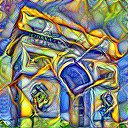
\includegraphics[width=\textwidth]{resources/gatys/architecture/sun-trees-paris-maxpool.png}
                \caption{Max pooling layers}
            \end{subfigure}
            \hfill
            \begin{subfigure}[b]{0.45\textwidth}
                \centering
                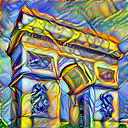
\includegraphics[width=\textwidth]{resources/gatys/architecture/sun-trees-paris-avgpool.png}
                \caption{Average pooling layers}
            \end{subfigure}
        \end{figure}

        Both results seems to be very good, but...
    \end{frame}
    
    \begin{frame}
        \begin{figure}[H]
            \centering
            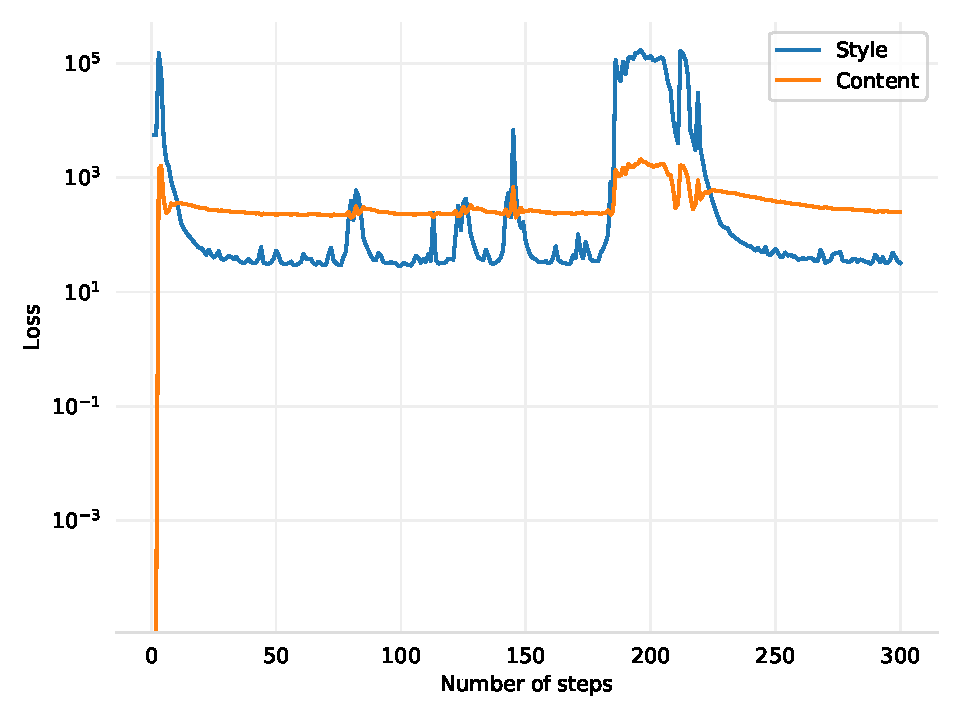
\includegraphics[width=0.6\textwidth]{resources/gatys/architecture/sun-trees-paris-avgpool.pdf}
            \caption*{Average pooling layers : loss functions}
        \end{figure}
        
        ...oscillations in loss functions ! \scriptsize{(which sometimes leads to bad results...)}
        
        \normalsize{We try to add a \textbf{scheduler} to reduce oscillations.}
    \end{frame}
    
    \begin{frame}
        \begin{figure}[H]
            \centering
            \begin{subfigure}[b]{0.40\textwidth}
                \centering
                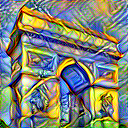
\includegraphics[width=\textwidth]{resources/gatys/architecture/sun-trees-paris-avgpool-scheduler.png}
                \caption{Average pooling layers}
            \end{subfigure}
            \hfill
            \begin{subfigure}[b]{0.50\textwidth}
                \centering
                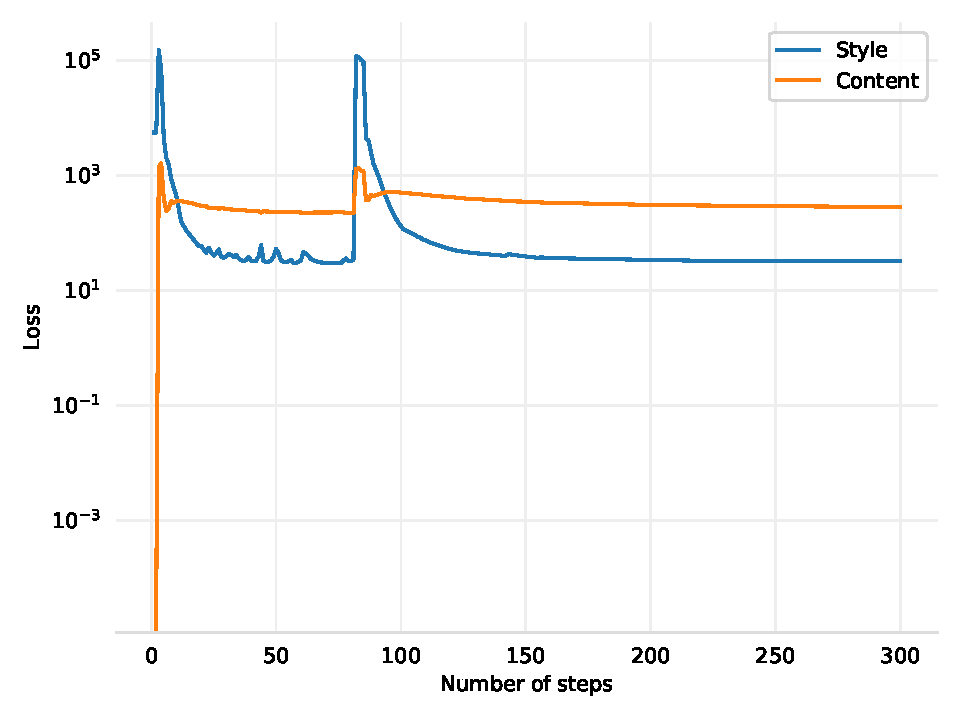
\includegraphics[width=\textwidth]{resources/gatys/architecture/sun-trees-paris-avgpool-scheduler.pdf}
                \caption{Loss functions with scheduler}
            \end{subfigure}
        \end{figure}
        
        Scheduler seems to be efficient !
        
        \footnotesize{Average pooling layers with scheduler chosen.}
    \end{frame}
    
    \begin{frame}{Weights}
        The $\alpha$ and $\beta$ weights in the loss function are used to distribute the style and content of the resulting image.
        $$\mathcal{L}_{total} = \alpha \mathcal{L}_{content} + \beta \mathcal{L}_{style}$$
        We set $\alpha$ to $10$ and try different ratios $\alpha/\beta$.
    \end{frame}
    
    \begin{frame}
        \begin{figure}[ht]
            \centering
            \begin{subfigure}[b]{0.25\textwidth}
                \centering
                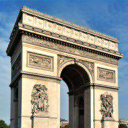
\includegraphics[width=\textwidth]{resources/gatys/weights/sun-trees-paris-10-2.png}
                \caption{$10^{-2}$}
            \end{subfigure}
            \hfill
            \begin{subfigure}[b]{0.25\textwidth}
                \centering
                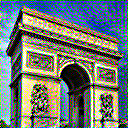
\includegraphics[width=\textwidth]{resources/gatys/weights/sun-trees-paris-10-3.png}
                \caption{$10^{-3}$}
            \end{subfigure}
            \hfill
            \begin{subfigure}[b]{0.25\textwidth}
                \centering
                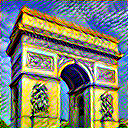
\includegraphics[width=\textwidth]{resources/gatys/weights/sun-trees-paris-10-4.png}
                \caption{$10^{-4}$}
            \end{subfigure}
            \begin{subfigure}[b]{0.25\textwidth}
                \centering
                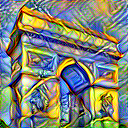
\includegraphics[width=\textwidth]{resources/gatys/weights/sun-trees-paris-10-5.png}
                \caption{$10^{-5}$}
            \end{subfigure}
            \hfill
            \begin{subfigure}[b]{0.25\textwidth}
                \centering
                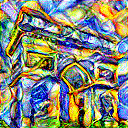
\includegraphics[width=\textwidth]{resources/gatys/weights/sun-trees-paris-10-6.png}
                \caption{$10^{-6}$}
            \end{subfigure}
            \hfill
            \begin{subfigure}[b]{0.25\textwidth}
                \centering
                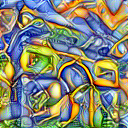
\includegraphics[width=\textwidth]{resources/gatys/weights/sun-trees-paris-10-7.png}
                \caption{$10^{-7}$}
            \end{subfigure}
        \end{figure}
        
        \footnotesize{Ratio $\alpha/\beta = 10^{-5}$ chosen (with $\alpha = 10$).}
    \end{frame}
    
    \begin{frame}{Added layers}
        The \textbf{positions of the construction layers in the network} have a significant influence on the result.
        
        We tried to place them at different locations to try to understand how they influence the result.
        \begin{figure}[H]
            \centering
            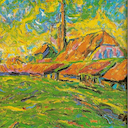
\includegraphics[width=0.3\textwidth]{resources/gatys/inputs/church.png}
            \caption*{Style used}
        \end{figure}
    \end{frame}
    
    \begin{frame}
        \begin{figure}[H]
            \centering
            \begin{subfigure}[b]{0.2\textwidth}
                \centering
                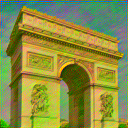
\includegraphics[width=\textwidth]{resources/gatys/layers/conv1_conv1.png}
                \caption{$s$: conv1  $c$: conv1}
            \end{subfigure}
            \hfill
            \begin{subfigure}[b]{0.2\textwidth}
                \centering
                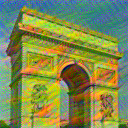
\includegraphics[width=\textwidth]{resources/gatys/layers/conv3_conv1.png}
                \caption{$s$: conv3 $c$: conv1}
            \end{subfigure}
            \hfill
            \begin{subfigure}[b]{0.2\textwidth}
                \centering
                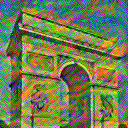
\includegraphics[width=\textwidth]{resources/gatys/layers/conv5_conv1.png}
                \caption{$s$: conv5 $c$: conv1}
            \end{subfigure}
            \hfill
            \begin{subfigure}[b]{0.2\textwidth}
                \centering
                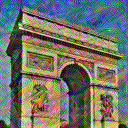
\includegraphics[width=\textwidth]{resources/gatys/layers/conv9_conv1.png}
                \caption{$s$: conv9 $c$: conv1}
            \end{subfigure}
            \begin{subfigure}[b]{0.2\textwidth}
                \centering
                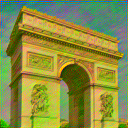
\includegraphics[width=\textwidth]{resources/gatys/layers/conv1_conv1.png}
                \caption{$s$: conv1  $c$: conv1}
            \end{subfigure}
            \hfill
            \begin{subfigure}[b]{0.2\textwidth}
                \centering
                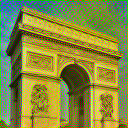
\includegraphics[width=\textwidth]{resources/gatys/layers/conv1_conv3.png}
                \caption{$s$: conv1 $c$: conv3}
            \end{subfigure}
            \hfill
            \begin{subfigure}[b]{0.2\textwidth}
                \centering
                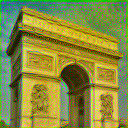
\includegraphics[width=\textwidth]{resources/gatys/layers/conv1_conv5.png}
                \caption{$s$: conv1 $c$: conv5}
            \end{subfigure}
            \hfill
            \begin{subfigure}[b]{0.2\textwidth}
                \centering
                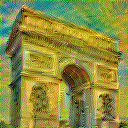
\includegraphics[width=\textwidth]{resources/gatys/layers/conv1_conv9.png}
                \caption{$s$: conv1 $c$: conv9}
            \end{subfigure}
        \end{figure}
        
        \footnotesize{Style layers placed at the beginning and content layer around the middle seems to be the best combination.}
    \end{frame}
    
    \begin{frame}
        \begin{figure}[H]
            \centering
            \begin{subfigure}[b]{0.45\textwidth}
                \centering
                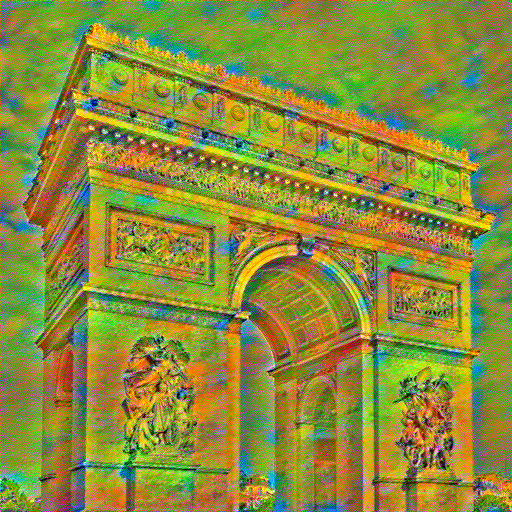
\includegraphics[width=\textwidth]{resources/gatys/layers/layers_default.png}
                \caption{Starting architecture}
            \end{subfigure}
            \hfill
            \begin{subfigure}[b]{0.45\textwidth}
                \centering
                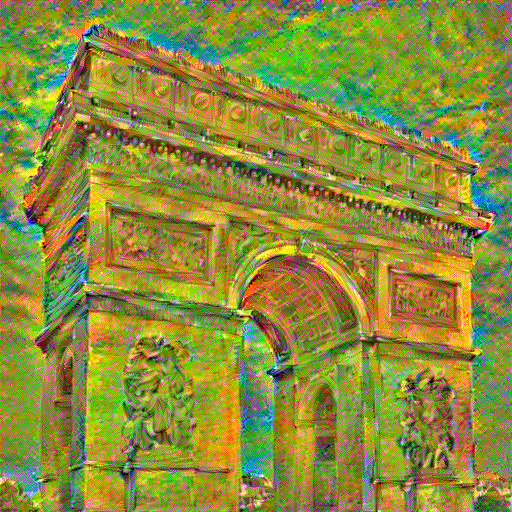
\includegraphics[width=\textwidth]{resources/gatys/layers/layers_nicer.png}
                \caption{Modified architecture}
            \end{subfigure}
        \end{figure}
        
        Result we obtained by modifying the locations of the construction layers.
    \end{frame}
    
    % ----- CycleGAN ----- %
    
    \section{CycleGAN (Zhu et al., 2017)}
    
    \begin{frame}{Introduction}
        CycleGAN allows \textit{unpaired image-image translation} using two Generative Adversarial Networks.
        
        \begin{figure}
            \centering
            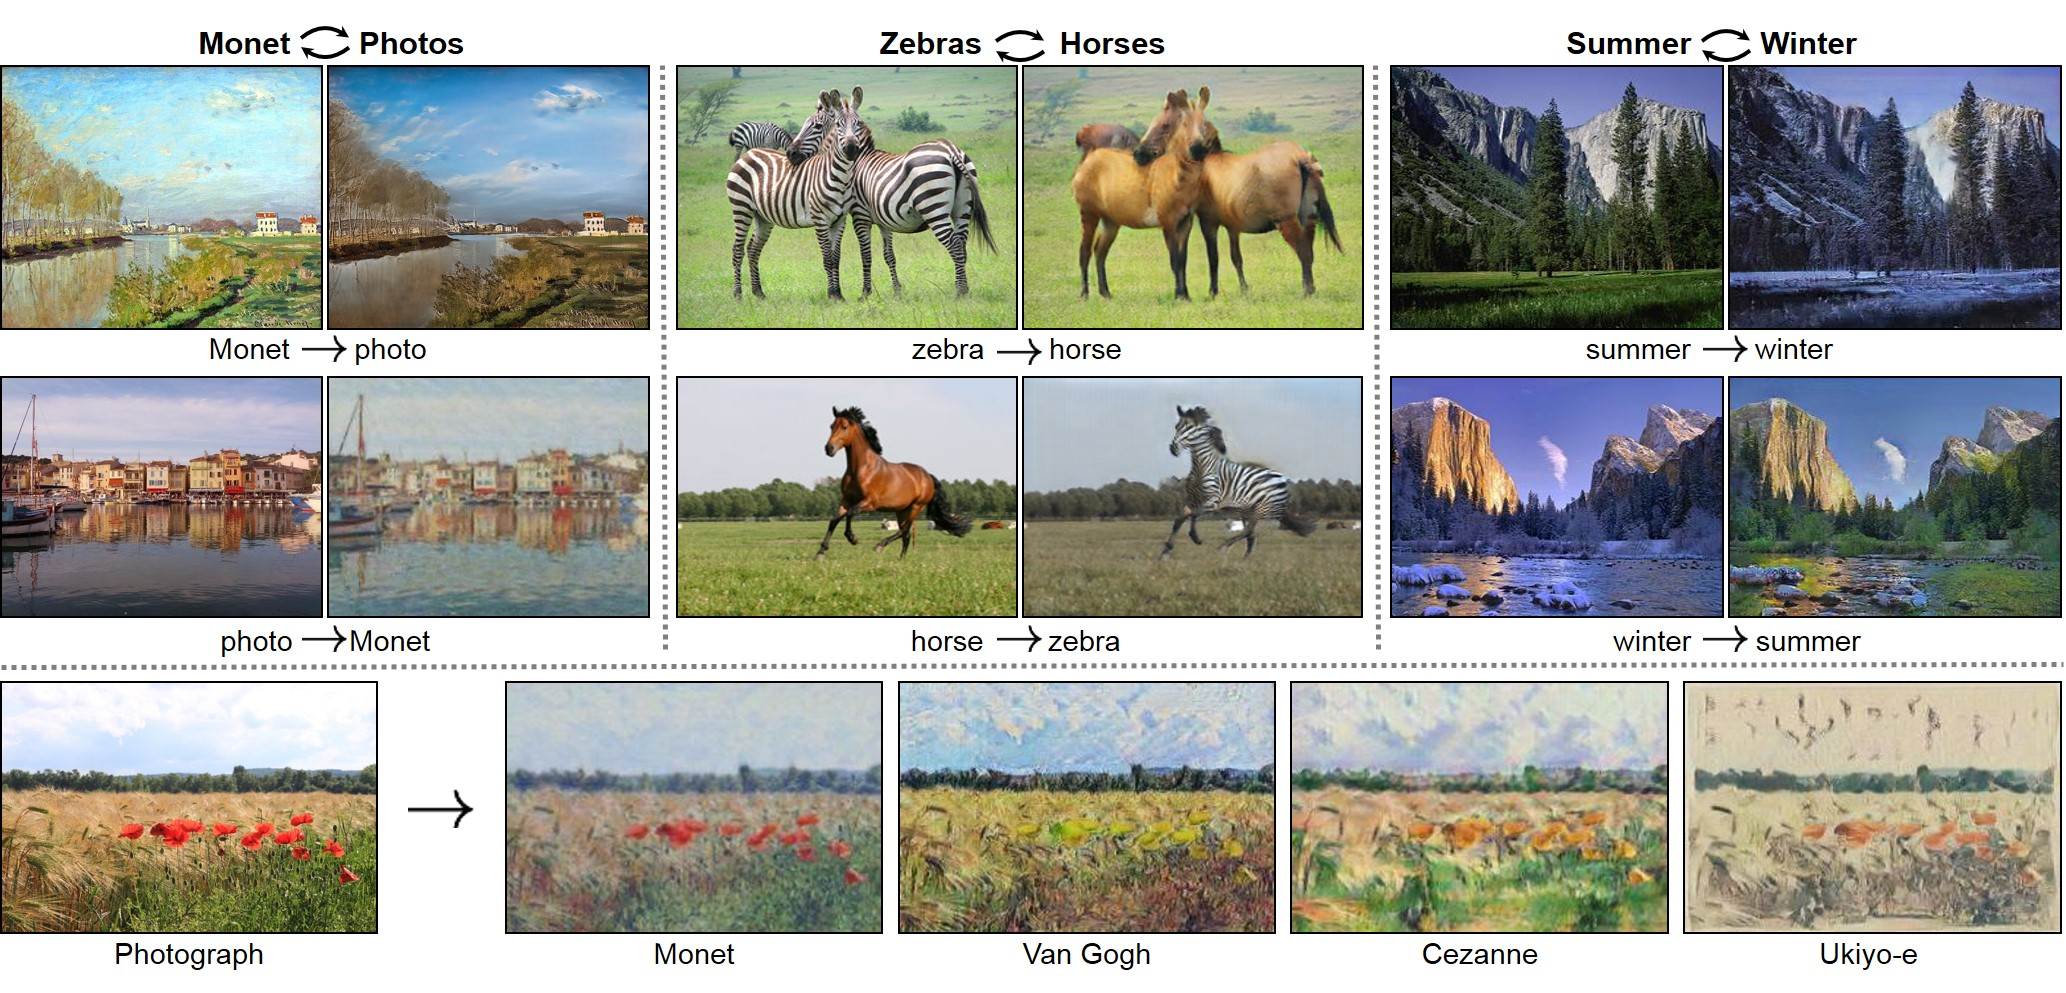
\includegraphics[scale=0.3]{resources/cycle-gan/cyclegan-examples.jpeg}
            \captionsource{Examples of CycleGAN applications}{https://junyanz.github.io/CycleGAN/}
        \end{figure}
    \end{frame}
    
    \begin{frame}{A word about GANs}
        \begin{itemize}
            \item \textbf{Generative} : Those models learn how to create data similar to what they have been fed.
            \item \textbf{Adversarial} : A generator and a discriminator compete.
        \end{itemize}

        \begin{figure}
            \centering
            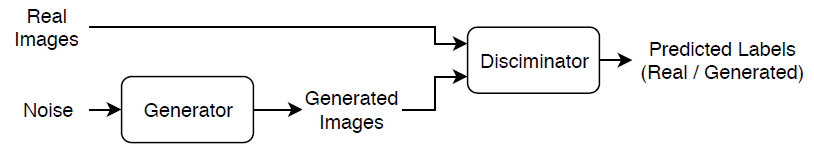
\includegraphics[scale=0.3]{resources/cycle-gan/gan-principles.png}
            \captionsource{GAN idea}{https://www.mathworks.com/help/deeplearning/ug/train-conditional-generative-adversarial-network.html}
        \end{figure}
    \end{frame}
    
    \begin{frame}{The idea of CycleGAN}
        Use two generators (one per domain) and two discriminators.
        
        The two generators should lead to bijection.
        
        $\longrightarrow$ \textbf{Cycle Consistency Loss} encouraging

        \begin{center}
            $F(G(x)) = x$ and $G(F(y)) = y$.
        \end{center}
        
        This helps avoid mode collapse.
    \end{frame}
    
    \begin{frame}{Losses}
        \begin{itemize}
            \item Adversarial loss (MSE in actual training): 
                \begin{align*}
                    \mathcal{L}_{\mathrm{GAN}}\left(G, D_{Y}, X, Y\right) &= \mathbb{E}_{y \sim p_{\text {data }}(y)}\left[\log D_{Y}(y)\right]\\
                    &+ \mathbb{E}_{x \sim p_{\text {data }}(x)}\left[\log \left(1-D_{Y}(G(x))\right]\right]
                 \end{align*}
            \item Cycle Consistency loss : 
                \begin{align*}
                    \mathcal{L}_{\text {cyc }}(G, F) &= \mathbb{E}_{x \sim p_{\text {data }}(x)}\left[\|F(G(x))-x\|_{1}\right]\\
                    &+ \mathbb{E}_{y \sim p_{\text {data }}(y)}\left[\|G(F(y))-y\|_{1}\right]
                \end{align*}
            \item Identity loss :
                \begin{align*}
                    \mathcal{L}_{\text {identity}}(G, F) &=\mathbb{E}_{y \sim p_{\text {data}}(y)}\left[\|G(y)-y\|_{1}\right] \\
                    &+\mathbb{E}_{x \sim p_{\text {data}}(x)}\left[\|F(x)-x\|_{1}\right]
                \end{align*}
        \end{itemize}
    \end{frame}
    
    \begin{frame}{Losses}
        Full loss :
        \begin{align*}
            \mathcal{L}\left(G, F, D_{X}, D_{Y}\right) &= \mathcal{L}_{\mathrm{GAN}}\left(G, D_{Y}, X, Y\right) + \mathcal{L}_{\mathrm{GAN}}\left(F, D_{X}, Y, X\right)\\
            &+ \lambda_{cyc} \mathcal{L}_{\mathrm{cyc}}(G, F) (+ \lambda_{id} \mathcal{L}_{\text {identity}}(G, F))
        \end{align*}
        Goal : 
        $$G^{*}, F^{*}=\arg \min _{G, F} \max _{D_{x}, D_{Y}} \mathcal{L}\left(G, F, D_{X}, D_{Y}\right)$$
    \end{frame}
    
    \begin{frame}{Architecture}
        \begin{figure}[H]
            \centering
            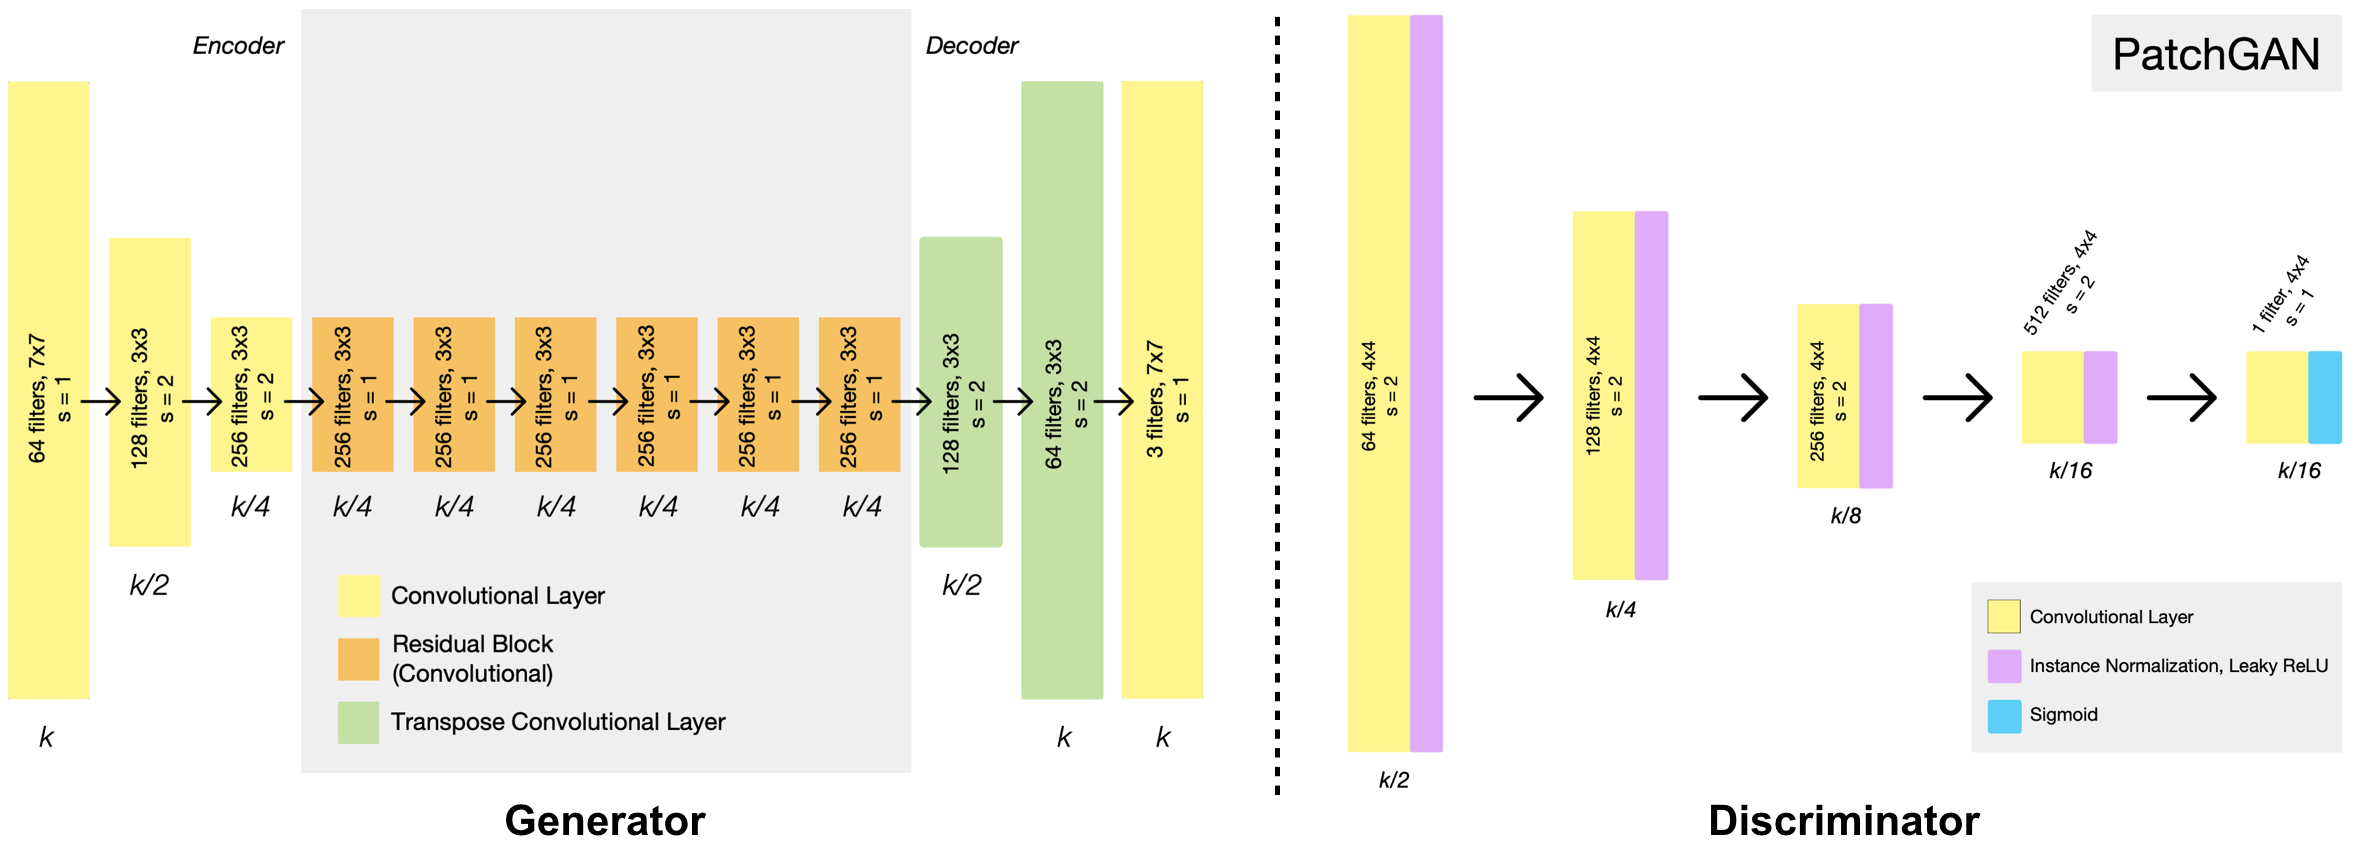
\includegraphics[scale=0.26]{resources/cycle-gan/gan-architecture.png}
            \captionsource{CycleGAN architecture}{https://www.lyrn.ai/2019/01/07/instagan-instance-aware-image-to-image-translation/}
        \end{figure}
    \end{frame}
    
    \begin{frame}{Input image}
        \begin{figure}[H]
            \centering
            \begin{subfigure}[b]{0.55\textwidth}
                \centering
                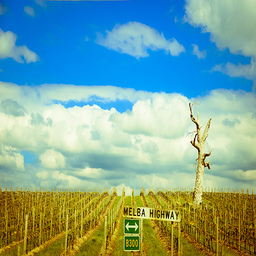
\includegraphics[width=\textwidth]{resources/cycle-gan/test4.jpg}
                \caption{Input image}
            \end{subfigure}
            \hfill
            \begin{subfigure}[b]{0.4\textwidth}
                \centering
                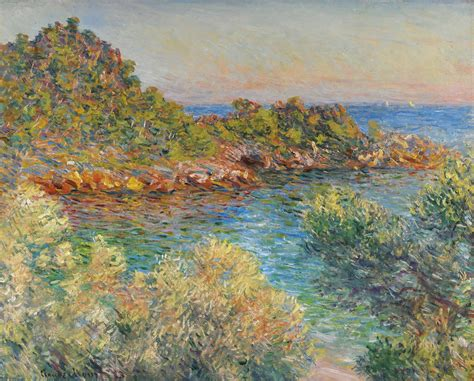
\includegraphics[width=\textwidth]{resources/cycle-gan/monet.png}
                \caption{Claude Monet, Près Monte-Carlo}
            \end{subfigure}
        \end{figure}
    \end{frame}
    
    \begin{frame}{Results}
        All training dataset (6000 + 1000 images) but limiting to 20 batches of 3 + 3 images per epoch :

        \begin{figure}[H]
            \centering
            \begin{subfigure}[b]{0.55\textwidth}
                \centering
                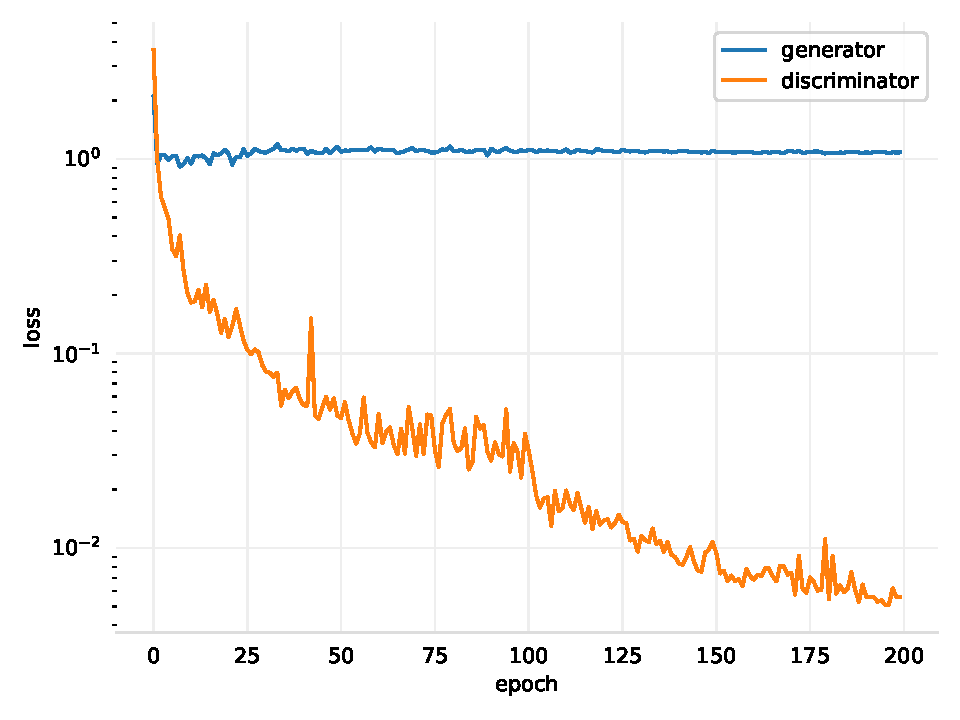
\includegraphics[width=\textwidth]{resources/cycle-gan/batch-limited.pdf}
                \caption{Losses for the limitation of batches}
            \end{subfigure}
            \hfill
            \begin{subfigure}[b]{0.4\textwidth}
                \centering
                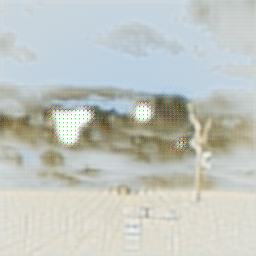
\includegraphics[width=\textwidth]{resources/cycle-gan/white.png}
                \caption{Result obtained}
            \end{subfigure}
        \end{figure}
    \end{frame}
    
    \begin{frame}{Results}
        Using only one model with identity loss (to avoid mode collapse) and plateau LR (0.01 and 0.0001):\footnote{Unless otherwise said, we used 120+750 images as training}
        
        \begin{figure}[H]
            \centering
            \begin{subfigure}[b]{0.3\textwidth}
                \centering
                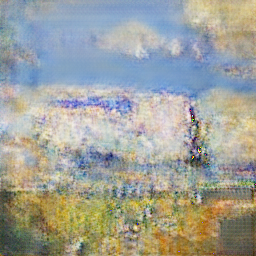
\includegraphics[width=\textwidth]{resources/cycle-gan/on100.png}
                \caption{Result for 100 epochs}
            \end{subfigure}
            \hfill
            \begin{subfigure}[b]{0.3\textwidth}
                \centering
                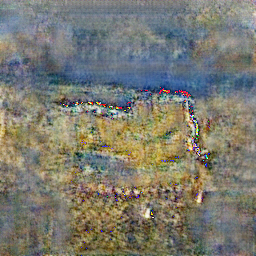
\includegraphics[width=\textwidth]{resources/cycle-gan/on.png}
                \caption{Result for 200 epochs}
            \end{subfigure}
            \begin{subfigure}[b]{0.3\textwidth}
                \centering
                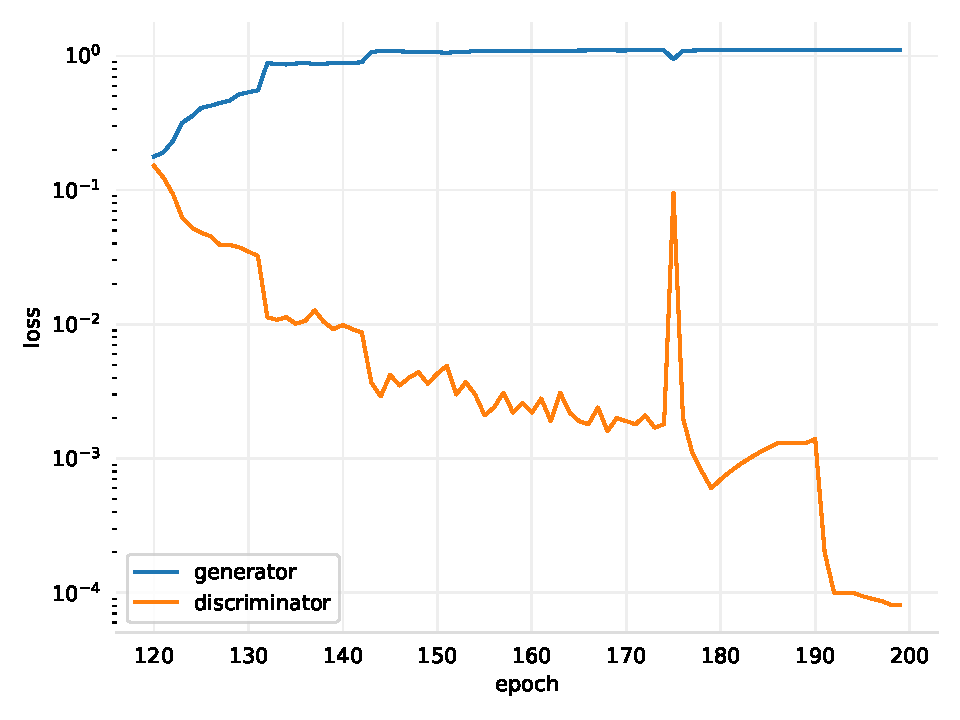
\includegraphics[width=\textwidth]{resources/cycle-gan/80.pdf}
                \caption{Losses}
            \end{subfigure}
            \hfill
        \end{figure}
    \end{frame}
    
    \begin{frame}{Other results}
        \begin{figure}[H]
            \centering
            \begin{subfigure}[b]{0.3\textwidth}
                \centering
                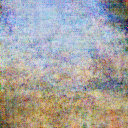
\includegraphics[width=\textwidth]{resources/cycle-gan/main10.png}
                \caption{$\lambda_{cyc}$ = 10 and dataset (50+150)}
            \end{subfigure}
            \hfill
            \begin{subfigure}[b]{0.3\textwidth}
                \centering
                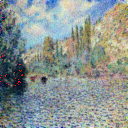
\includegraphics[width=\textwidth]{resources/cycle-gan/main1.png}
                \caption{$\lambda_{Id} = \lambda_{Cyc} = 1$}
            \end{subfigure}
            \hfill
            \begin{subfigure}[b]{0.3\textwidth}
                \centering
                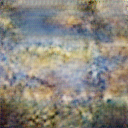
\includegraphics[width=\textwidth]{resources/cycle-gan/main3.png}
                \caption{Reduce LR on Plateau (0.001)}
            \end{subfigure}
            \begin{subfigure}[b]{0.3\textwidth}
                \centering
                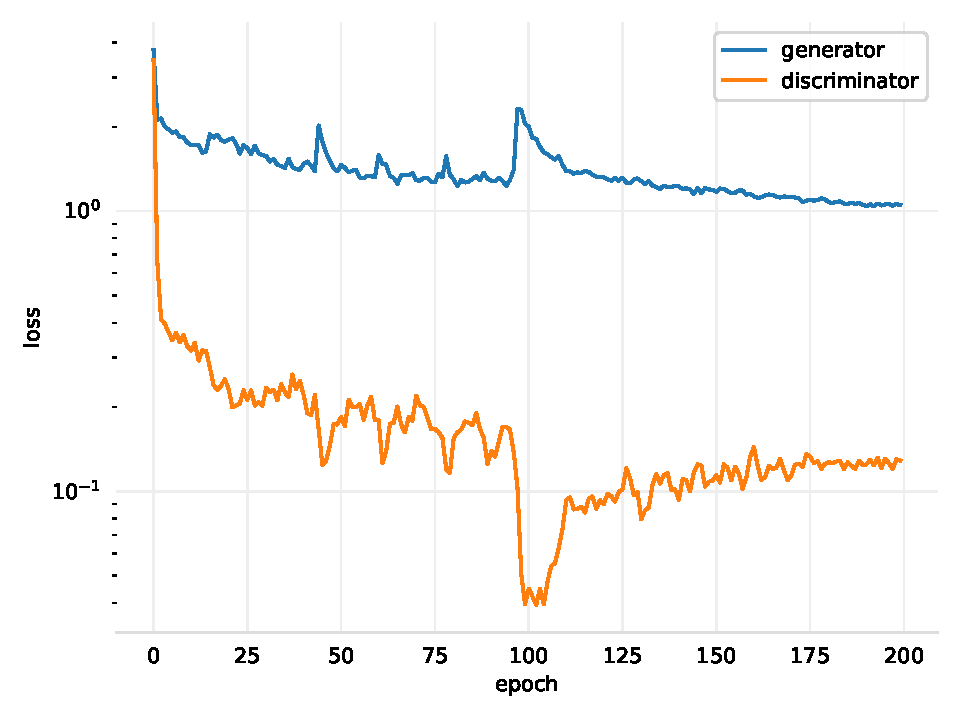
\includegraphics[width=\textwidth]{resources/cycle-gan/main10.pdf}
            \end{subfigure}
            \hfill
            \begin{subfigure}[b]{0.3\textwidth}
                \centering
                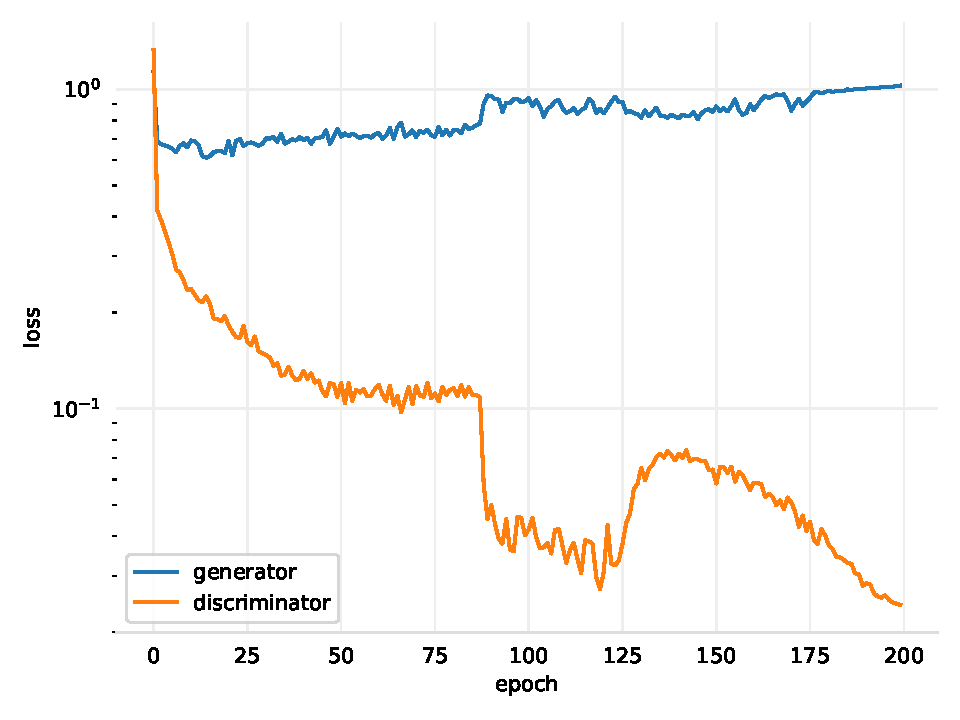
\includegraphics[width=\textwidth]{resources/cycle-gan/main.pdf}
            \end{subfigure}
            \hfill
            \begin{subfigure}[b]{0.3\textwidth}
                \centering
                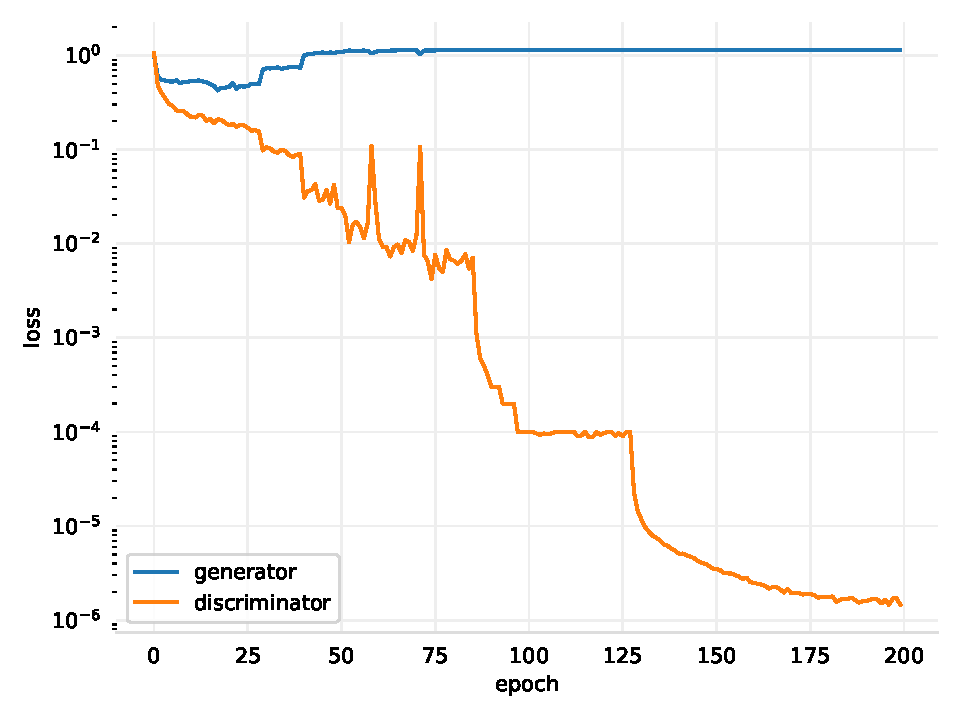
\includegraphics[width=\textwidth]{resources/cycle-gan/main3.pdf}
            \end{subfigure}
            \hfill
        \end{figure}
    \end{frame}
    
    \begin{frame}{Other results}
        \begin{minipage}{0.5\textwidth}
            \begin{figure}[H]
                \begin{subfigure}[b]{\textwidth}
                    \centering
                    \includegraphics[width=\textwidth]{resources/cycle-gan/main6.png}
                    \caption{Result at 160 epochs}
                \end{subfigure}
            \end{figure}
        \end{minipage}
        \hfill
        \begin{minipage}{0.45\textwidth}
            \begin{itemize}
                \item $\lambda_{id} = \lambda_{cyc} = 1$
                \item 5 training of discriminators per training of generators
                \item Clamping parameters of discriminators between -0.01 and 0.01
            \end{itemize}
        \end{minipage}
    \end{frame}

    % ----- Conclusion ----- %
    
    \section{Conclusion}
    
    \begin{frame}{A Neural Algorithm of Artistic Style}
        \begin{itemize}
            \item Results of Gatys et al.'s technique look very good
            \item Loss functions stabilize quickly
            \item Many improvements are now possible
        \end{itemize}
        
        \vspace{2em}
        
        \begin{itemize}
            \item Does not generalize directly...
            \item ...but gives results very quickly !
        \end{itemize}
    \end{frame}
    
    \begin{frame}{CycleGAN}
        \begin{itemize}
            \item Good results are very hard to obtain
            \item Probably caused by a dataset not big enough
            \item The long training time (3-5 days) made it lengthy to tweak
            \item Using only one GAN could be enough for the task
        \end{itemize}
    \end{frame}
    
    \begin{frame}{Comparison}
        \begin{table}[H]
            \centering
            \footnotesize{
                \begin{tabular}{l|p{3cm}|p{3cm}}
                    & \textbf{NAoAS}\footnote{A Neural Algorithm of Artistic Style} & \textbf{CycleGAN}\\ \hline
                    \hline
                    \textbf{Scope of the tool} & Specific to one style image but easily adapted & General (style of an artist) but limited (one style per training)\\ \hline
                    \textbf{Training} & Just needs a pre-trained model \scriptsize{(instantaneous with tools like PyTorch)} & Requires lots of time and resources\\ \hline
                    \textbf{Results} & Works on the fly, needs to tweak parameters each time & Better, more natural results than NAoAS \scriptsize{(but harder to get...)}\\ \hline
                \end{tabular}
            }
        \end{table}
    \end{frame}
    
    % ----- End of the presentation ----- %
    
    \begin{frame}[standout]
        \footnotesize{Our journey ends here... but we have only opened the first door to the world of neural style transfer !}

        \Large{Thank you for your attention !}
    \end{frame}
    
    % ----- References ----- %

    \begin{frame}[allowframebreaks]
        \nocite{*}
        \printbibliography
    \end{frame}
    
    % ----- Additional resources ----- %
    
    \section{Additional resources}
    
    \begin{frame}{CNN structure}
        \begin{figure}[H]
            \centering
            \includegraphics[width=0.9\textwidth]{resources/additional/cnn-structure.png}
            \captionsource{CNN structure}{https://cutt.ly/nyL20Qo}
        \end{figure}
    \end{frame}
    
    \begin{frame}{CNN layers}
        A CNN is generally composed of 3 types of layer :

        \begin{itemize}
            \item \textbf{convolutional layer} : apply a filter to its input (to get a so called \textit{feature map})
            \item \textbf{pooling layer} : aggregate values in a local region (non trainable, used to reduce size)
            \item \textbf{fully-connected layer} : combine features in a non-linear way
        \end{itemize}
    \end{frame}
    
    \begin{frame}{Gram matrices}
        In NAoAS, why the Gram matrices could represent style ? \footnotesize{Well, it's pretty mysterious...}
        
        \normalsize{
            This article\footnote{\url{https://arxiv.org/pdf/1701.01036.pdf}} tries to demystify it.
            
            In particular, they show that \emph{matching the Gram matrices of feature maps is equivalent to minimize the Maximum Mean Discrepancy (MMD) with the second order polynomial kernel.}
        }
        
        \footnotesize{$\longrightarrow$ The essence of neural style transfer is to match the feature distributions between the style images and the generated images.}
    \end{frame}
    
    \begin{frame}{Maximum Mean Discrepancy (MMD)}
        The MMD statistic can be used to \textbf{measure the difference between two distributions}.
        
        \footnotesize{
            \begin{align*}
                \text{MMD}^{2}[X, Y] &= \left\|E_{x}[\phi(x)]-E_{y}[\phi(y)]\right\|^{2}\\
                &= \left\|\frac{1}{n} \sum_{i=1}^{n} \phi\left(x_{i}\right)-\frac{1}{m} \sum_{j=1}^{m} \phi\left(y_{j}\right)\right\|^{2}\\
                &= ...\\
                &= \frac{1}{n^2}\sum_{i=1}^n\sum_{i'=1}^n k(x_i, x_{i'}) + \frac{1}{m^2}\sum_{j=1}^m\sum_{j'=1}^m k(y_j, y_{j'})\\
                &- \frac{2}{nm}\sum_{i=1}^n\sum_{j=1}^m k(x_i, y_{j})
            \end{align*}
        }
    \end{frame}
    
    \begin{frame}{Auto-encoders}
        \footnotesize{\emph{According to the theoretical course,}}\footnote{\url{https://glouppe.github.io/info8010-deep-learning/?p=lecture7.md\#7}}
        
        \normalsize{
            An auto-encoder is a composite function made of
            
            \begin{itemize}
                \item an encoder $f$ from the original space $\mathcal{X}$ to a latent space $\mathcal{Z}$,
                \item a decoder $g$ to map back to $\mathcal{X}$,
            \end{itemize}
            
            such that $g \circ f$ is close to the identity on the data.
        }
    \end{frame}
    
    \begin{frame}{Auto-encoders and CycleGAN}
        \footnotesize{\emph{According to the original paper,}}\footnote{\url{https://arxiv.org/pdf/1703.10593.pdf}}
        
        \normalsize{
            CycleGAN modal can be viewed as 2 auto-encoders :
            
            \begin{itemize}
                \item one auto-encoder $F \circ G : X \rightarrow X$ jointly with
                \item another auto-encoder $G \circ F : Y \rightarrow Y$
            \end{itemize}
        }
        
        \scriptsize{Special internal structures : they map an image to itself via an intermediate representation that is a translation of the image into another domain.}
    \end{frame}
    
    \begin{frame}{CycleGAN architecture}
        \begin{itemize}
            \item Generator :
            \begin{center}
                \footnotesize{\texttt{c7s1-64,d128,d256,[R256](6 or 9),u128,u64,c7s1-3(Tanh)}}
            \end{center}
            \item Discriminator :
            \begin{center}
                \footnotesize{\texttt{C64-C128-C256-C512-C512(stride 1)-Conv2d}}
            \end{center}
        \end{itemize}
        
        \footnotesize{
            \texttt{c} : \texttt{ConvInstanceNormRelu}
            
            \texttt{d} : same but stride of $2$
            
            \texttt{R} : residual block
            
            \texttt{u} : same as \texttt{c} but with stride $1/2$
            
            \texttt{C} : \texttt{ConvInstanceNormLeakyRelu} with stride $2$
        }
    \end{frame}
\end{document}
